
\subsection{Construcción del sistema}\label{sec:construccion}

El sistema se construyó con tres piezas de bajo costo (cuadro~\ref{tab:piezas}):
una placa ESP32-CAM, un adaptador USB-serial y un computador portátil. La placa
lleva el sensor de imagen y un microcontrolador, pero no tiene puerto USB; por
eso se conecta al computador mediante el adaptador, que traduce el puerto serial
(UART) de la placa al USB del computador (figura~\ref{fig:hardware}).

\begin{figure}[htbp]
\centering
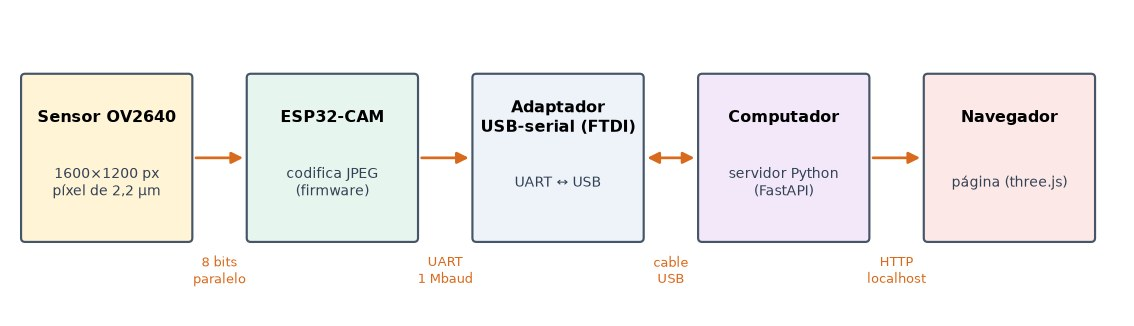
\includegraphics[width=\linewidth]{hardware_bloques.jpg}
\caption{Construcción del sistema: el sensor entrega los píxeles a la ESP32-CAM, que
los comprime a JPEG y los envía por el cable USB al servidor; la página web los
muestra y recibe el modelo 3D.}
\label{fig:hardware}
\end{figure}

\begin{table}[htbp]
\caption{Piezas del sistema y sus datos principales}
\label{tab:piezas}
\centering\small
\begin{tabular}{@{}p{3.6cm}p{4.4cm}p{6.2cm}@{}}
\toprule
Pieza & Qué hace & Dato principal \\
\midrule
Sensor OV2640 & Convierte la luz en una matriz de píxeles & $1\,600\times1\,200$ píxeles, píxel de $2{,}2\ \mu$m, área de $3{,}59\times2{,}68$ mm \citep{omnivision} \\
ESP32-CAM (AI Thinker) & Lee el sensor, comprime a JPEG y envía los bytes & Dos núcleos, memoria PSRAM externa, sin puerto USB propio \citep{aithinker} \\
Adaptador USB-serial (FTDI FT232R) & Pasa la señal UART al USB & Velocidad usada: $1\,000\,000$ baudios \\
Computador portátil & Ejecuta el servidor (Python) y la página web & Procesador de 8 núcleos, sin tarjeta gráfica dedicada \\
\bottomrule
\end{tabular}
\end{table}

\paragraph{Firmware.} La ESP32-CAM se programó con un firmware propio
(\texttt{firmware/camara\_esp32}). Al arrancar configura el sensor para entregar
JPEG, con un reloj de $20$ MHz, resolución SVGA ($800\times600$ píxeles) y
calidad de compresión 10, y guarda dos cuadros a la vez en la memoria PSRAM para
leer uno mientras el sensor captura el siguiente. Después repite sin parar: toma
el cuadro más reciente y escribe sus bytes, tal cual, en el puerto serial.
También acepta comandos de un carácter (por ejemplo, \texttt{h} y \texttt{v}
activan el espejo horizontal y el volteo vertical del sensor), que la página usa
para enderezar la imagen.

\paragraph{Protocolo y velocidad.} Cada cuadro es un archivo JPEG completo, que
siempre empieza con los bytes \texttt{FF D8} y termina con \texttt{FF D9}; el
servidor corta el flujo de bytes en esos marcadores y obtiene un cuadro por
cada par. El puerto serial usa 8 bits de datos, sin paridad y 1 bit de parada:
cada byte viaja con $10$ bits (los 8 de datos más el de inicio y el de parada).
Con $B$ baudios, la capacidad del cable es
\begin{equation}
\text{bytes por segundo} = \frac{B}{10} = \frac{1\,000\,000}{10} = 100\,000,
\qquad
\text{cuadros por segundo} \le \frac{100\,000}{S},
\end{equation}
donde $S$ es el tamaño del cuadro en bytes. Un cuadro de $47\,020$ bytes, como
el que se midió en las pruebas, permite como máximo $100\,000/47\,020\approx2{,}1$
cuadros por segundo; como el tamaño del JPEG cambia con la escena, el promedio
medido fue de $17$ cuadros en $6$ segundos, unos $2{,}8$ por segundo. A
$2\,000\,000$ baudios los cuadros llegaban con bytes dañados y no se podían decodificar,
por eso se dejó $1\,000\,000$.

\subsection{Adquisición de los datos: de la luz a la matriz $I$}\label{sec:adquisicion}

Esta sección sigue el camino de un dato, desde que la luz llega al sensor hasta
que el programa tiene la matriz de la foto. Todos los números son de la foto del
casco (sección «\nameref{sec:casco}»).

\paragraph{1. El sensor.} Cada píxel del sensor mide cuánta luz recibe a través
de un filtro rojo, verde o azul. Con la cámara ESP32-CAM se puede pedir $800\times600$
píxeles (SVGA) o hasta $1\,600\times1\,200$ (UXGA). La distancia focal en píxeles
depende de la resolución: con el ángulo de visión horizontal $\alpha=65^\circ$
que usa el programa, $f=(W/2)/\tan(\alpha/2)$ vale $627{,}874$ píxeles a $800$ de ancho,
$753{,}449$ a $960$ y $1255{,}7$ a $1\,600$. En milímetros, esa focal corresponde a
$1255{,}7\times2{,}2\ \mu\text{m}\approx2{,}76$ mm. Las hojas de datos de módulos con este
sensor traen focales entre $3{,}6$ y $4{,}2$ mm \citep{microchip,arducam}; con el ancho del sensor
($3{,}59$ mm), $2\arctan\bigl(1{,}795/f_{\text{mm}}\bigr)$ da ángulos de visión horizontales entre unos $46^\circ$ y $53^\circ$.
Por eso el valor de $65^\circ$ es una suposición del programa y no una medida de la cámara (se podría
afinar calibrándola), y es una de las razones por las que el tamaño en milímetros del modelo es aproximado
(limitaciones, sección de discusión): con un ángulo menor, la misma foto corresponde a una focal mayor y a puntos 3D más grandes.

\paragraph{2. De bytes a matriz: el JPEG.} Los bytes que llegan por el cable son
una imagen comprimida. Para volver a la matriz $I$ hay que deshacer tres
transformaciones, y las tres son productos de matrices cuya inversa se conoce:
\begin{enumerate}
  \item \textbf{Transformada del coseno (DCT).} La foto se corta en bloques de
        $8\times8$ píxeles. Para cada bloque $X$ (valores de brillo menos $128$) el
        compresor guarda la matriz de coeficientes
        \begin{equation}
        Y = C\,X\,C^{T},\qquad
        C_{kj}=\alpha_k\cos\frac{(2j+1)k\pi}{16},\quad
        \alpha_0=\sqrt{\tfrac18},\ \alpha_k=\tfrac12\ (k\ge1),
        \end{equation}
        donde $C$ es de $8\times8$. Esa matriz es \emph{ortogonal}: $CC^T=I$, así que
        su inversa es su transpuesta, y el decodificador recupera el bloque con
        $X=C^{T}\,Y\,C$. Con un bloque real del casco (la unión entre la visera oscura y la mentonera clara,
        columnas $480$--$487$ y filas $694$--$701$ de la foto):
        \begin{equation*}
        X=\begin{pmatrix} 3 & 3 & 3 & 4 & 4 & 4 & 3 & 2 \\ 10 & 8 & 6 & 6 & 5 & 4 & 5 & 5 \\ 58 & 51 & 44 & 39 & 34 & 30 & 24 & 20 \\ 93 & 84 & 72 & 63 & 58 & 55 & 55 & 54 \\ 204 & 193 & 178 & 162 & 148 & 141 & 133 & 123 \\ 248 & 249 & 249 & 246 & 242 & 238 & 237 & 233 \\ 229 & 230 & 233 & 236 & 238 & 239 & 237 & 236 \\ 238 & 237 & 237 & 238 & 237 & 237 & 235 & 235 \end{pmatrix} ,\qquad
        Y=\begin{pmatrix} -36 & 57 & 6 & 6 & 0 & 2 & 0 & 0 \\ -780 & 5 & 5 & 1 & 1 & 0 & 0 & 0 \\ -4 & -61 & -13 & -4 & 2 & -1 & 1 & -1 \\ 147 & 0 & -5 & -2 & -2 & 1 & -1 & 1 \\ -54 & 24 & 9 & 2 & -1 & 0 & 0 & 0 \\ -33 & -22 & -1 & 0 & 1 & -1 & 0 & 0 \\ 58 & 4 & -4 & -1 & 0 & 0 & 0 & 0 \\ 4 & 24 & -2 & 4 & -1 & 1 & 1 & -1 \end{pmatrix} .
        \end{equation*}
        El coeficiente $Y_{10}=-780$ es el más grande: el bloque pasa de oscuro
        (arriba) a claro (abajo), que es la frecuencia vertical más baja. Aplicando
        $C^{T}YC$ y sumando $128$ se recupera $X$ con un error máximo de
        $1{,}4\times10^{-13}$ (solo redondeo del computador), y se comprueba $\max|CC^T-I|=6{,}7\times10^{-16}$.
  \item \textbf{De YCbCr a RGB.} El JPEG guarda el brillo $Y'$ y dos diferencias de
        color $C_b,C_r$ (cada una en $[0,255]$, con $128$ como cero) mediante una matriz de $3\times3$:
        \begin{equation}
        \begin{pmatrix}Y'\\C_b-128\\C_r-128\end{pmatrix}=
        \underbrace{\begin{pmatrix} 0{,}299000 & 0{,}587000 & 0{,}114000 \\ -0{,}168736 & -0{,}331264 & 0{,}500000 \\ 0{,}500000 & -0{,}418688 & -0{,}081312 \end{pmatrix}}_{T}\begin{pmatrix}R\\G\\B\end{pmatrix},\qquad
        T^{-1}=\begin{pmatrix} 1 & 0 & 1{,}402 \\ 1 & -0{,}344 & -0{,}714 \\ 1 & 1{,}772 & 0 \end{pmatrix} .
        \end{equation}
        La inversa $T^{-1}$ se calcula con el mismo método de Gauss--Jordan de la
        sección «\nameref{sec:inversa}». Para el píxel B de la foto, $(R,G,B)=\begin{pmatrix} 231 \\ 231 \\ 243 \end{pmatrix}$ da
        $(Y',C_b,C_r)=\begin{pmatrix} 232{,}37 \\ 134 \\ 127{,}02 \end{pmatrix}$, y al multiplicar por $T^{-1}$ se recupera $(R,G,B)=\begin{pmatrix} 231 \\ 231 \\ 243 \end{pmatrix}$.
  \item \textbf{Cuantización.} Los coeficientes se redondean al comprimir; esta es la única
        pérdida de información, y la controla el parámetro de calidad.
\end{enumerate}
El resultado es la matriz $I\in\{0,\dots,255\}^{H\times W\times3}$: una matriz de
$H\times W$ entradas, cada una un vector $(r,g,b)\in\mathbb{R}^3$.

\begin{figure}[htbp]
\centering
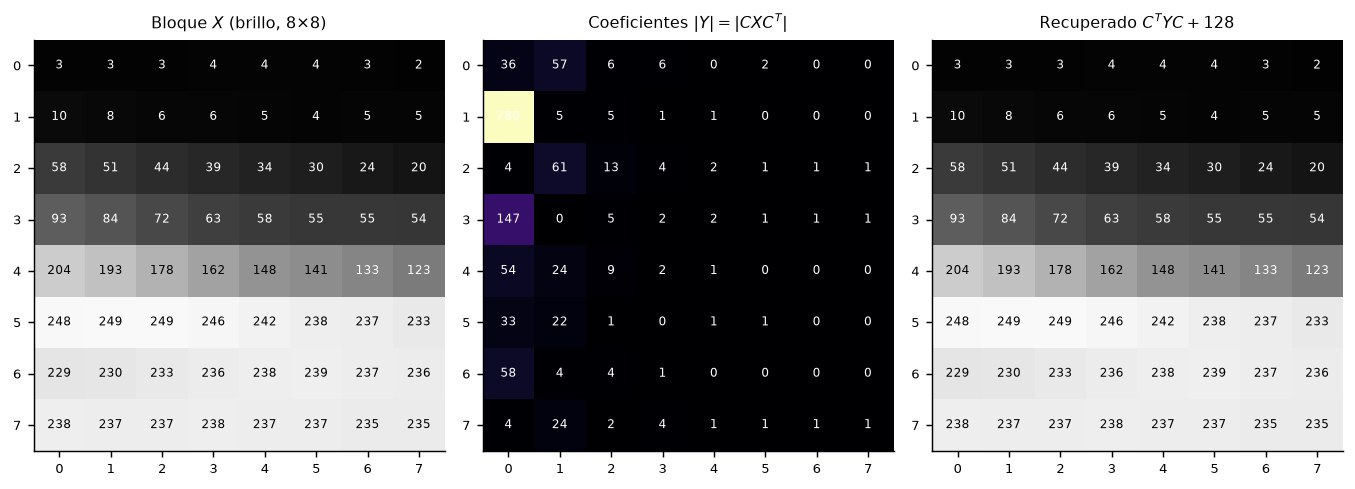
\includegraphics[width=\linewidth]{casco_dct.jpg}
\caption{Bloque de $8\times8$ píxeles del casco (izquierda), su matriz de
coeficientes $Y=CXC^T$ (centro, en valor absoluto) y el bloque recuperado con
$C^{T}YC$ (derecha): la inversa de una matriz ortogonal es su transpuesta.}
\label{fig:dct}
\end{figure}

\paragraph{3. Reducción de tamaño.} Antes de calcular, la foto se reduce al ancho de
procesamiento $960$ píxeles. Con el factor $s=960/1200=0{,}8$, cada píxel nuevo es el promedio
ponderado por área de los píxeles que cubre, que es una combinación lineal de
las entradas de $I$. La foto de $1200\times1600$ queda de $960\times1280$ píxeles
(cada píxel nuevo cubre $1/s^2=1{,}5625$ píxeles originales).

\paragraph{4. Los números de entrada.} La matriz reducida $I'$ tiene
$1280\cdot960=1\,228\,800$ píxeles y $3\,686\,400$ números. Los tres píxeles que se siguen en
todo el desarrollo son (figura~\ref{fig:casco-entrada}):
\begin{center}\small
\begin{tabular}{cccc}
\toprule
Píxel & $(u,v)$ & Lugar en la foto & $(R,G,B)$ \\
\midrule
A & $(488,\,576)$ & centro de la visera (oscuro) & $\begin{pmatrix} 1 \\ 1 \\ 1 \end{pmatrix}$ \\
B & $(450,\,300)$ & parte superior del casco (blanco) & $\begin{pmatrix} 231 \\ 231 \\ 243 \end{pmatrix}$ \\
C & $(221,\,576)$ & borde izquierdo de la máscara & $\begin{pmatrix} 199 \\ 143 \\ 90 \end{pmatrix}$ \\
\bottomrule
\end{tabular}
\end{center}
La distancia entre dos colores es la norma de la diferencia de sus vectores:
$\lVert c_A-c_B\rVert=\lVert\begin{pmatrix} -230 \\ -230 \\ -242 \end{pmatrix}\rVert=405{,}4$, que es grande porque A es casi negro y B casi
blanco, mientras que B y un píxel vecino dan una norma cercana a cero.
